\documentclass[a4paper]{standalone}
\usepackage{amsmath}
\usepackage{circuitikz}
\usetikzlibrary{fit, shapes, arrows, patterns, decorations.text, decorations.markings}

\begin{document}
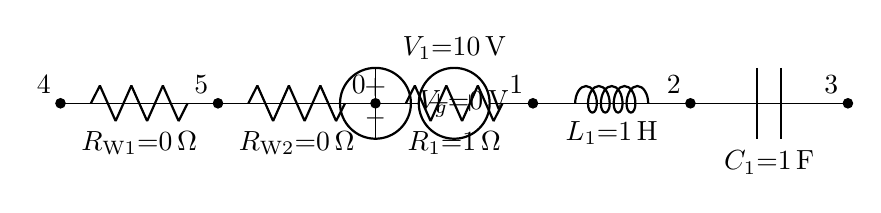
\begin{tikzpicture}[scale=1.00, transform shape, /tikz/circuitikz/bipoles/length=1.50cm, american currents, american voltages, voltage dir=RP]
  \coordinate (0) at (4,0);
  \coordinate (1) at (6,0);
  \coordinate (2) at (8,0);
  \coordinate (3) at (10,0);
  \coordinate (4) at (0,0);
  \coordinate (5) at (2,0);
  \draw (0) to [R, l_={$R_{1}$=$1\,\mbox{$\Omega$}$}, n=R1] (1);
  \draw (1) to [L, l_={$L_{1}$=$1\,\mbox{H}$}, n=L1] (2);
  \draw (2) to [C, l_={$C_{1}$=$1\,\mbox{F}$}, n=C1] (3);
  \draw (3) to [V, l_={$V_{1}$=$10\,\mbox{V}$}, n=V1] (4);
  \draw (4) to [R, l_={$R_{\mathrm{W1}}$=$0\,\mbox{$\Omega$}$}, n=RW1] (5);
  \draw (5) to [R, l_={$R_{\mathrm{W2}}$=$0\,\mbox{$\Omega$}$}, n=RW2] (0);
  \draw (0) to [V, l_={$V_{g}$=$0\,\mbox{V}$}, n=Vg] (0);
  \draw (0) node[circ] {};
  \draw (1) node[circ] {};
  \draw (2) node[circ] {};
  \draw (3) node[circ] {};
  \draw (4) node[circ] {};
  \draw (5) node[circ] {};
  \draw[anchor=south east] (0) node {0};
  \draw[anchor=south east] (1) node {1};
  \draw[anchor=south east] (2) node {2};
  \draw[anchor=south east] (3) node {3};
  \draw[anchor=south east] (4) node {4};
  \draw[anchor=south east] (5) node {5};
\end{tikzpicture}
\end{document}